\chapter{Planung der Funktionstest-Anwendung} \label{PlanungAnwendung}

Anhand des durch die Anforderungsanalyse festgelegten Rahmens müssen nun Entscheidungen bezüglich Tests der Datenhaltung, der Sensoren und des Designs der Benutzeroberfläche und Benutzerführung getroffen werden. In den folgenden Abschnitten werden diese Entscheidungen behandelt. Wie schon in Kapitel \ref{Anforderungsanalyse} erläutert, wird die Funktionstest-Anwendung zunächst als Referenz für die Plattform Android nativ entwickelt. Entsprechend wird sich unter anderem bei der graphischen Benutzeroberfläche an den Android Guidelines orientiert, welche im Folgenden näher erläutert werden. 

\section{GUI Design} \label{PlanungAnwGUI}

Die Android GUI-Guidelines beschreiben das Design-Prinzip von Android Anwendungen als 'Material Design'. Das Design, die Oberfläche soll materiell, greifbar wirken. Der Gebrauch von gewohnten, greifbaren Attributen soll dem Benutzer helfen schnell Funktionen und Bedienelemente zu verstehen. Licht, Oberflächenbeschaffen-heiten und Bewegung beschreiben wie einzelne Objekte Der GUI miteinander interagieren und in welcher Relation sie zueinander stehen. Die fundamentalen Elemente print-basierten Designs wie die Typographie, Raum, Farbe und Metaphorik dienen nicht nur optischen Highlights sondern sie formen Hierarchien, Bedeutung und Fokus. Im Material Design soll so eine Oberfläche geschaffen werden, die als 'bold and graphic' bezeichnet wird. Diese zeichnen gezielte Farbkombinationen, bewusst eingesetzte Leerräume und eine groß-skalierte Typographie aus. Die Bewegungen einzelner Bedienelemente sollen bedeutungsvoll sein und dazu dienen den Fokus auf sich zu ziehen um den Benutzer auf intuitive Art und Weise durch Anwendungen navigieren zu lassen. Auf diese weise soll auch klar verständliches Feedback auf Benutzereingaben gegeben werden\footcite{AndroidOnlineGuidelines}. 
\\
\\
Die Android Design-Guidelines betonen folgende 3 Prinzipien:

\begin{itemize}
\item Enchant Me
\begin{list}{}{}
\item Mit 'Enchant Me' ist gemeint, dass zum Beispiel vorsichtig platzierte Animationen und gut gesetzte Soundeffekte dafür sorgen, dem Benutzer ein Gefühl von Mühelosigkeit vermitteln sollen. Dem Benutzer soll die Möglichkeit gegeben werden anstelle von Buttons und Menüs direkt mit einzelnen Objekten in der Anwendung interagieren zu können. Dies soll die kognitive Anstrengung gering halten und die Anwendung ansprechender gestalten. Mit der Möglichkeit optionaler Anpassungen soll der Benutzer der Anwendung eine persönliche Note geben können. Zudem sollte eine Anwendung lernen, was die Präferenzen des Benutzers sind und entsprechende häufig verwendete Funktionen in den Vordergrund heben und leicht erreichbar anbieten\footcite{AndroidDesignPrinciples}.
\end{list}
\item Simplify My Life
\begin{list}{}{}
\item Unter 'Simplify My Life' zählt unter anderem, dass darauf geachtet werden sollte, kurze Sätze mit einfachen Wörtern zu verwenden, da lange Sätze eher eine abschreckende Wirkung haben. Zudem sollten, wo es nur möglich ist, Bilder und Symbole anstelle von Text genutzt werden, um Ideen zu erklären. Einstellbare, bzw. konfigurable Funktionen sollten voreingestellt sein, um den Benutzer vor der ersten Nutzung der Anwendung einen Einstellungsmarathon zu ersparen. Es sollte dem Benutzer aber die Möglichkeit gegeben werden die Konfigurationen einfach nach seinem Geschmack anzupassen. Für eine bessere Übersichtlichkeit sollte auch darauf geachtet werden nicht zu viele Optionen und Informationen gleichzeitig anzuzeigen und so die Anzeige zu überladen und den Benutzer zu überfordern. Verschiedene Bereiche in einer Anwendung sollen verschieden aussehen und es sollen Übergänge zwischen Bereichen geschaffen werden, die deren Beziehungen untereinander verdeutlichen. Auf diese Weise soll der Benutzer die Orientierung in der Anwendung nicht verlieren. Des weiteren soll darauf geachtet werden, dass Formen, hinter denen bestimmte Funktionen stecken, ausschließlich für diese Funktionen genutzt werden, frei nach dem Motto 'Was gleich aussieht, sollte gleich funktionieren'. Als letztes wird unter dem Punkt 'Simplify My Life' aufgeführt, dass der Benutzer nur dann bei der Bedienung unterbrochen werden soll, wenn diese Unterbrechung dazu dient wirklich kritische Informationen zu übermitteln. Wegen unnötiger Details sollte der Benutzer nicht gestört werden\footcite{AndroidDesignPrinciples}. 
\end{list}
\item Make Me Amazing
\begin{list}{}{}
\item 'Make Me Amazing' besagt unter anderem, dass man versuchen sollte visuelle und haptische Muster und Gesten aus anderen Android Anwendungen in die eigene Anwendung mit einfließen zu lassen. So hat es der Benutzer nochmals leichter sich in der neuen Anwendung zurecht zu finden. Werden von dem Benutzer Korrekturen verlangt, so sollten diese ihm freundlich vermittelt werden. Wenn etwas schief läuft, sollen klare ver-ständliche Wiederherstellungsanweisungen gegeben werden, auf technische Details sollte verzichtet werden. Alles was im Hintergrund ohne den Benutzer ablaufen kann, sollte dort geschehen. Auf sämtlichen Benutzereingaben sollte es ein Feedback geben, auch wenn es nur ein leichtes leuchten ist. Können mehrere komplizierte Arbeitsschritte zusammengefasst werden, sollte man dies tun und es dem Benutzer als Bündel zur Verfügung stellen. Ein Beispiel hierfür wären einige kombinierte Filter für die Fotonachbereitung. Zu guter Letzt wird darauf hingewiesen, dass darauf geachtet werden soll, dass die wichtigsten Funktionen der Anwendung leicht zu finden und zu benutzen sein sollen. Als gutes Beispiel dient hier der Pause-Button bei Musik-Anwendungen oder der Auslöser bei der Kamera\footcite{AndroidDesignPrinciples}. 
\end{list}
\end{itemize}

Für die geplante Funktionstest-Anwendung bedeutet dies, dass zumindest die Standard 'Material Design' Bedien- und Navigationselemente integriert werden sollten. Das Android Studio bietet einige Kompositionen an Elementen für die Seitenerstellung an, an diese sollte sich gehalten werden, da sie dem 'Material Design'-Prinzip entsprechen. Zu diesen Elementen zählen zum Beispiel der 'Navigation Drawer' für die Navigation zwischen einzelnen Seiten der Anwendung oder der 'Floating Action Button', ein runder Button, welcher im Vordergrund über dem Inhalt der Anwendung schwebt. Er verschwindet nicht, wenn hinter ihm in der Seite gescrollt wird und steht so immer zur Verfügung. Auch die 'Bottom Navigation Bar' darf in der Anwendung nicht fehlen, sie ist eine einheitliche globale Navigation durch das Android Betriebssystem. Auch eine 'App Bar' soll am oberen Rand des Displays integriert werden. Diese stellt Shortcuts und weitere Menüverwaltungsmöglichkeiten zur Verfügung. In unten stehender Abbildung \ref{fig:Material_Design} ist eine leere Beispielseite einer Android Anwendung im 'Material Design' Abgebildet. Man erkennt deutlich die 'Bottom Navigation Bar' am unteren Rand der Seite, die 'App Bar' am oberen Rand und den 'Floating Action Button' in der rechten unteren Ecke. 

\begin{figure}[h]
	\centering
	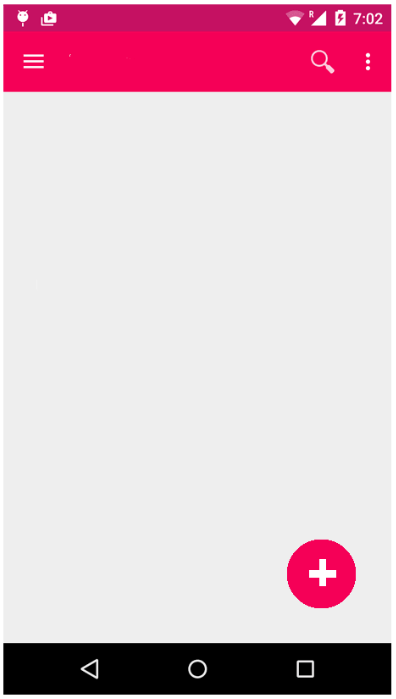
\includegraphics[width=0.35\textwidth]{Bilder/Material_Design_Blank_Page.PNG}
	\caption{Beispiel einer leeren Seite einer Android Anwendung im 'Material Design'}
	\label{fig:Material_Design}
\end{figure}

\section{Hardwarezugriffe}

Android bietet für den Zugriff auf Sensoren auf der API-Ebene im Paket android.hardware Unterstützung für eine Vielzahl von Sensoren an. In der Sensor-Klasse ist für jeden Sensortyp eine Konstante definiert, wie zum Beispiel \\ Sensor.TYPE\_ACCELEROMETER für den Beschleunigungssensor. Einige dieser Sensoren repräsentieren dabei tatsächliche Hardware-Sensoren, andere wiederum sind Software-basierte Sensoren, deren Messungen auf einer Kombination von Hardware-Sensoren basieren\footcite{Android5}. Da es Smartphones gibt die pro Sensortyp mit mehreren Sensoren ausgestattet sein können, gibt es pro Typ in Android einen sogenannten Default-Sensor und eine Sensorliste, in welcher alle verfügbaren Sensoren eines Typs enthalten sind. Über den Reporting-Mode kann eingestellt werden, wann der Sensor Daten an die Anwendung liefern soll. Hier gibt es unter anderem die Möglichkeit kontinuierlich Daten übermitteln zu lassen oder nur bei Änderungen in der Messung\footcite{AndroidQuickAPI}. 
\\
\\
Für die Standortbestimmung bietet Android eine eigene, separate API. Aufgrund datenschutzrechtlicher Bestimmungen müssen bei der Standortbestimmung Berechtigungen direkt vom Benutzer eingeholt werden um diese nutzen zu können. Die eigentliche Bestimmung des Standortes kann auf 3 unterschiedliche Weisen geschehen: einmal via GPS, via WiFi Zugangspunkten oder Sendemasten oder als dritte Möglichkeit passiv über die Standortanfragen anderer auf dem Smartphone befindlicher Anwendungen\footcite{AndroidQuickAPI}. 
\\
\\
Für die Interaktion mit den Kameras des Smartphones bietet Android ein reichhaltiges Set an APIs. Ähnlich zur Standortbestimmung werden auch bei der Nutzung der Kameras Berechtigungen gefordert. Der Entwickler kann im Manifest seiner Android Anwendung einstellen, ob die Kameranutzung für die Anwendung notwendig oder optional ist. Eine Anwendung, für die die Kameranutzung notwendig ist, kann über Google Play nicht auf Geräten ohne Kamera installiert werden. Android stellt zudem noch einige Konfigurationsparameter bereit, über die sich zum Beispiel die Qualität des JPEG-Bildes oder Blitzfunktionen voreinstellen lassen\footcite{AndroidQuickAPI}. 

\section{Speicher} \label{PlanungAnwSpeicher}

Für das Speichern von Daten gibt es je nach Zweck und Datengröße unterschiedliche Möglichkeitnen bei Android. So können zu jeder Activity über sogenannte Shared Preferences Konfigurationen gespeichert werden. Die auf diese Weise gespeicherten Daten sind Privateigentum der jeweiligen Activity, keine andere Activity oder gar Anwendung hat Zugriff darauf\footcite{Android5}. 
\\
\\
Bei größeren Datenmengen und für direktes Lesen und Schreiben in Dateien ist der Shared Preferences Ansatz eher ungeeignet. Hier werden Java-IO-Klassen wie zum Beispiel der FileInpuStream oder der FileOutputStream verwendet. Als Speicherorte gibt es den internen Speicher (Internal Storage) und den externen Speicher (External Storage)\footcite{Android5}:

\begin{itemize}
\item Interner Speicher:
\begin{list}{}{}
\item Der interne Speicher ist immer vorhanden, die enthaltenen Daten sind Anwendungs-spezifisch. Dies bedeutet, dass nur die Anwendung, der die Daten gehören Zugriff auf diese besitzt. Andere Anwendungen können diese Daten nicht nutzen. Wird die Anwendung deinstalliert, so werden in diesem Zuge auch alle Daten in ihrem internen Speicher gelöscht\footcite{Android5}. 
\end{list}
\item Externer Speicher:
\begin{list}{}{}
\item Daten im externen Speicher können von mehreren Anwendungen genutzt werden. Der externe Speicher kann in Form einer einsteckbaren SD-Karte vorliegen, aber auch der Speicher des Smartphones hat einen Bereich, der als 'External Storage' angesprochen werden kann. Je nach Android-Version gibt es allerdings Unterschiede bezüglich der Zugriffsrechte und der Unterteilung des Speichers\footcite{Android5}. 
\end{list}
\end{itemize}

In der Funktionstest-Anwendung soll die Verwendung des externen Speichers innerhalb des Smartphones, also ohne extra SD-Karte integriert werden. Hierbei soll sowohl das Lesen als auch das Schreiben von Dateien umgesetzt werden. 